%% Author_tex.tex
%% This file describes the coding for IET.cls

\documentclass{IET}%%%%where IET is the template name

%The authors can define any packages after the \documentclass{IET} command.

%Some of the packages are:
%\usepackage{hyperref} for linking the cross references
%\usepackage{graphics} for dealing with figures.
%\usepackage{algorithmic} for describing algorithms
\usepackage{fixltx2e}
\usepackage{hyperref}
\usepackage{capt-of}
\usepackage{pgffor}
\usepackage{gensymb}
%The author can find the documentation of the above style file and any additional
%supporting files if required from "http://www.ctan.org"

% *** Do not adjust lengths that control margins, column widths, etc. ***

\newtheorem{theorem}{Theorem}
\newtheorem{condition}{Condition}

\newcommand{\fourPic}{0.225}
\newcommand{\threePic}{0.32}
\newcommand{\twoPic}{0.45}
\newcommand{\onePic}{2\twoPic}
\newcommand{\real}{\mathbb{R}}

\begin{document}

\title{A face classifer for North Atlantic Right whales}

\author[1,*]{Matt Smith}
\affil{Department of Statistics, University of Warwick, Coventry, United Kingdom}

\author{Abhir Bhalerao}
%%%% By default, the citations will come automatically,
%%%% The optional bracket "[2.*]" is used  to display the corresponding author symbol
\affil{Department of Computer Science, University of Warwick, Coventry, United Kingdom}

\author{Ben Graham}
\affil{Facebook Artificial Intelligence Research, Paris, France}
%%%% Corresponding author detail must placed here
\affil[*]{m.d.smith@warwick.ac.uk}

\abstract{Accurate monitoring of individuals in a threatened species is of upmost importance to conservationists and researchers. Human observation is expensive and autonomous ariel photography is becoming an increasingly useful technique regarding animal biometrics \cite{koh2012dawn,martin2012estimating}. Fewer than 500 North Atlantic right whales are left in the world's oceans. As with many animal biometric inspection processes, tracking and monitoring individuals is an extremely time consuming process. Advances in the implementation and performance of deep learning algorithms have drastically improved performance in object detection and recognition tasks \cite{lecun2015deep}.  We employ a wide range of interesting techniques to build a "face-identification" algorithm for ariel photos of 447 unique. We follow a conventional modern face recognition pipeline consisting of the stages: detect, align, represent and classify \cite{taigman2014deepface}. We use deep learning algorithms to both detect and classify. A fully convolutional network \cite{long2015fully} is employed to semantically segment a given image to detect the location of the whale's head and body, we then use PCA on the resulting image to normalize for the whale's direction. A significant amount of hand labelled masks are needed to generate enough supervised training data to make this work effectively \cite{hong2015decoupled}. We tackle this issue by employing semi-supervised learning techniques and histogram matching between images to improve our localization algorithm and find a significant improvement in our results.}

\maketitle

\section{Introduction}
We entered the 2015 Right Whale Recognition online competition issued by Kaggle. Data consists of aeriel images, the vast majority containing a single Right whale. There are $M$ = 447 unique whales, each of which has at least one photo in the training set which contains 4543 labelled images. The test set contains $N$ = 6925 unlabelled images. Evaluation is based on the multi-class logarithmic loss
\begin{eqnarray}
\text{logloss} = - \frac{1}{N} \sum_{i=1}^{N} \sum_{i=1}^{M} y_{ij} \text{log}(p_{ij}),
\end{eqnarray}
where log is the natural logarithm, $y_{ij}$ is 1 if observation $i$ belongs to whale $j$ and 0 otherwise, and $p_{ij}$ is the predicted probability that observation $i$ belongs to whale $j$. 

The data was collected and labelled over a 10 year period by NOAA (National Oceanic and Atmospehric Administration) scientists via numerous helicopter trips over the northern Atlantic. 

We follow the conventional pipeline of alignment and classification and break our task of classifying a given photo, denoted $X_i$ into two main stages, both of which employ using convolutional neural networks;
\begin{itemize}
\item Alignment - We first reduce the dimensionality of $X_i$ and normalize for the distance to and orientation of the whale, generating a headshot of the whale, denoted $X_i^h$.
\item Classification - $X_i^h$ is passed through a classifier which outputs a probability mass function over the 447 whales.
\end{itemize}

\subsection{Related work}
Subsection text here.

\section{Alignment}

It is helpful to remove variation in inputs before giving them to a deep learning algorithm and, especially with faces, the success of a learned network is highly dependant on an alignment step \cite{lecun2012efficient,taigman2014deepface}. 

\subsubsection{Mask prediction}

We randomly choose 550 images from our training set $M^{Train}$ and another random 150 images to generate a test set $M^{Test}$. Using a graphics editor, for each $X_i \in {M^{Train}, M^{Test}}$ we create a semantic mask denoted $M_i$. An example of a pair is shown in figure \ref{fig:whaleLabel}.
\begin{figure}[H]
\centering     %%% not \center
\subfigure[]{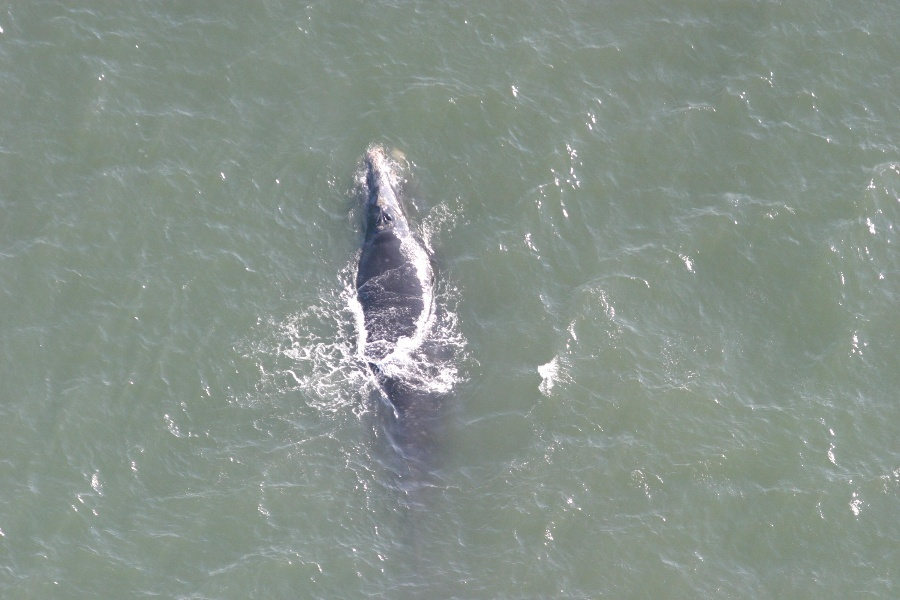
\includegraphics[width=0.45\textwidth]{images/maskExample/x.jpg}}
\subfigure[]{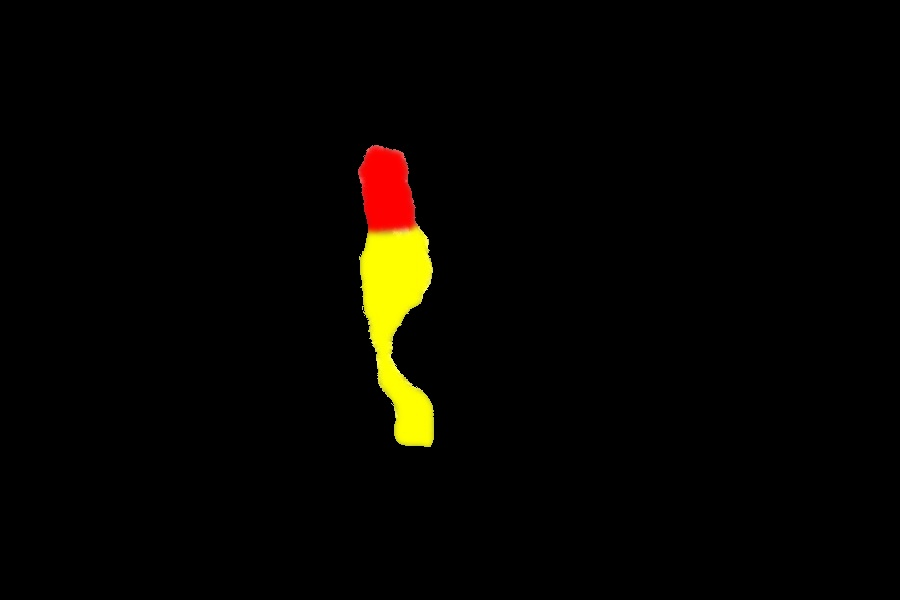
\includegraphics[width=0.45\textwidth]{images/maskExample/y.jpg}}
\caption{Example of $\{X_i,M_i\}$ pair;\
a) $X_i$, b) $M_i$.
}\label{fig:whaleLabel}
\end{figure}
We distinguish between head, body and sea using red, yellow and black respectivley. Having two colors for distinguishing parts of the whale enables us to infer the direcition in which the whale is pointing. We rescale each $X_i$ to dimension $w \times h \times c = 600 \times 900 \times 3$ and each $M_i$ to $w^{'}\times h^{'}\times c^{'} = 19 \times 29 \times 3$. We further process $X_i$ as described later on, creating $X_i^1$ and feed it into a fully connected convolutional neural network (FCNN) to learn a function $f_1: \real^{w\times h \times c} \to \real^{w^{'}\times h^{'}\times c^{'}}$. We are not interested in a huge amount of detail being produced in our predicted $\hat{M}_i$, enough to infer head and body location, hence our choice for relatively small output space.

We describe our neural network architecture as follows;
\begin{align}\label{eq:whaleconv1}
	 f_1 = \{X_i^1 - \text{down\textsubscript{0}} - , ... , - \text{down\textsubscript{4}} - 3\text{C}_{2D}3/1 - \text{sigmoid}\ - \hat{M}_i \}, 
\end{align}
	where 
\begin{align}
			 \text{conv\textsubscript{n}} &= \{(48 + 32\text{n})\text{C}_{2D}3/1 - \text{BN} - \text{ReLU}\}, \\	
     		 \text{down\textsubscript{n}}  &= \{\text{conv\textsubscript{n}}- \text{MP}3/2\}.
     		 \label{eq:whaleconv1block}
\end{align}
The following notation for denoting a network architecture is similar to \cite{graham2014fractional}. $\{a-b-c-d\}$ denotes a network where the intial tensor $a$ is passed through the layers $b$, the output of which is passed through $c$ finally creating output $d$. $fC_{iD}k/s$ denotes an $i$ dimensional convolutional layer with kernel size $k$ in each dimension, a stride of $s$ and number of filters $f$. Similarly MP$k/s$ is a two dimensional max-pooling layer with kernel size $k$ and stride $s$. Other layer notations; BN $=$ batch normalization, ReLU and Sigmoid are layers of rectified linear activation units and sigmoid activation units respectively. An illustration w of $f_1$ is given in figure \ref{fig:nn}.

\begin{figure}
\centering
\begin{minipage}[t]{0.6\textwidth}
\centering
\vspace{0pt}
\centering
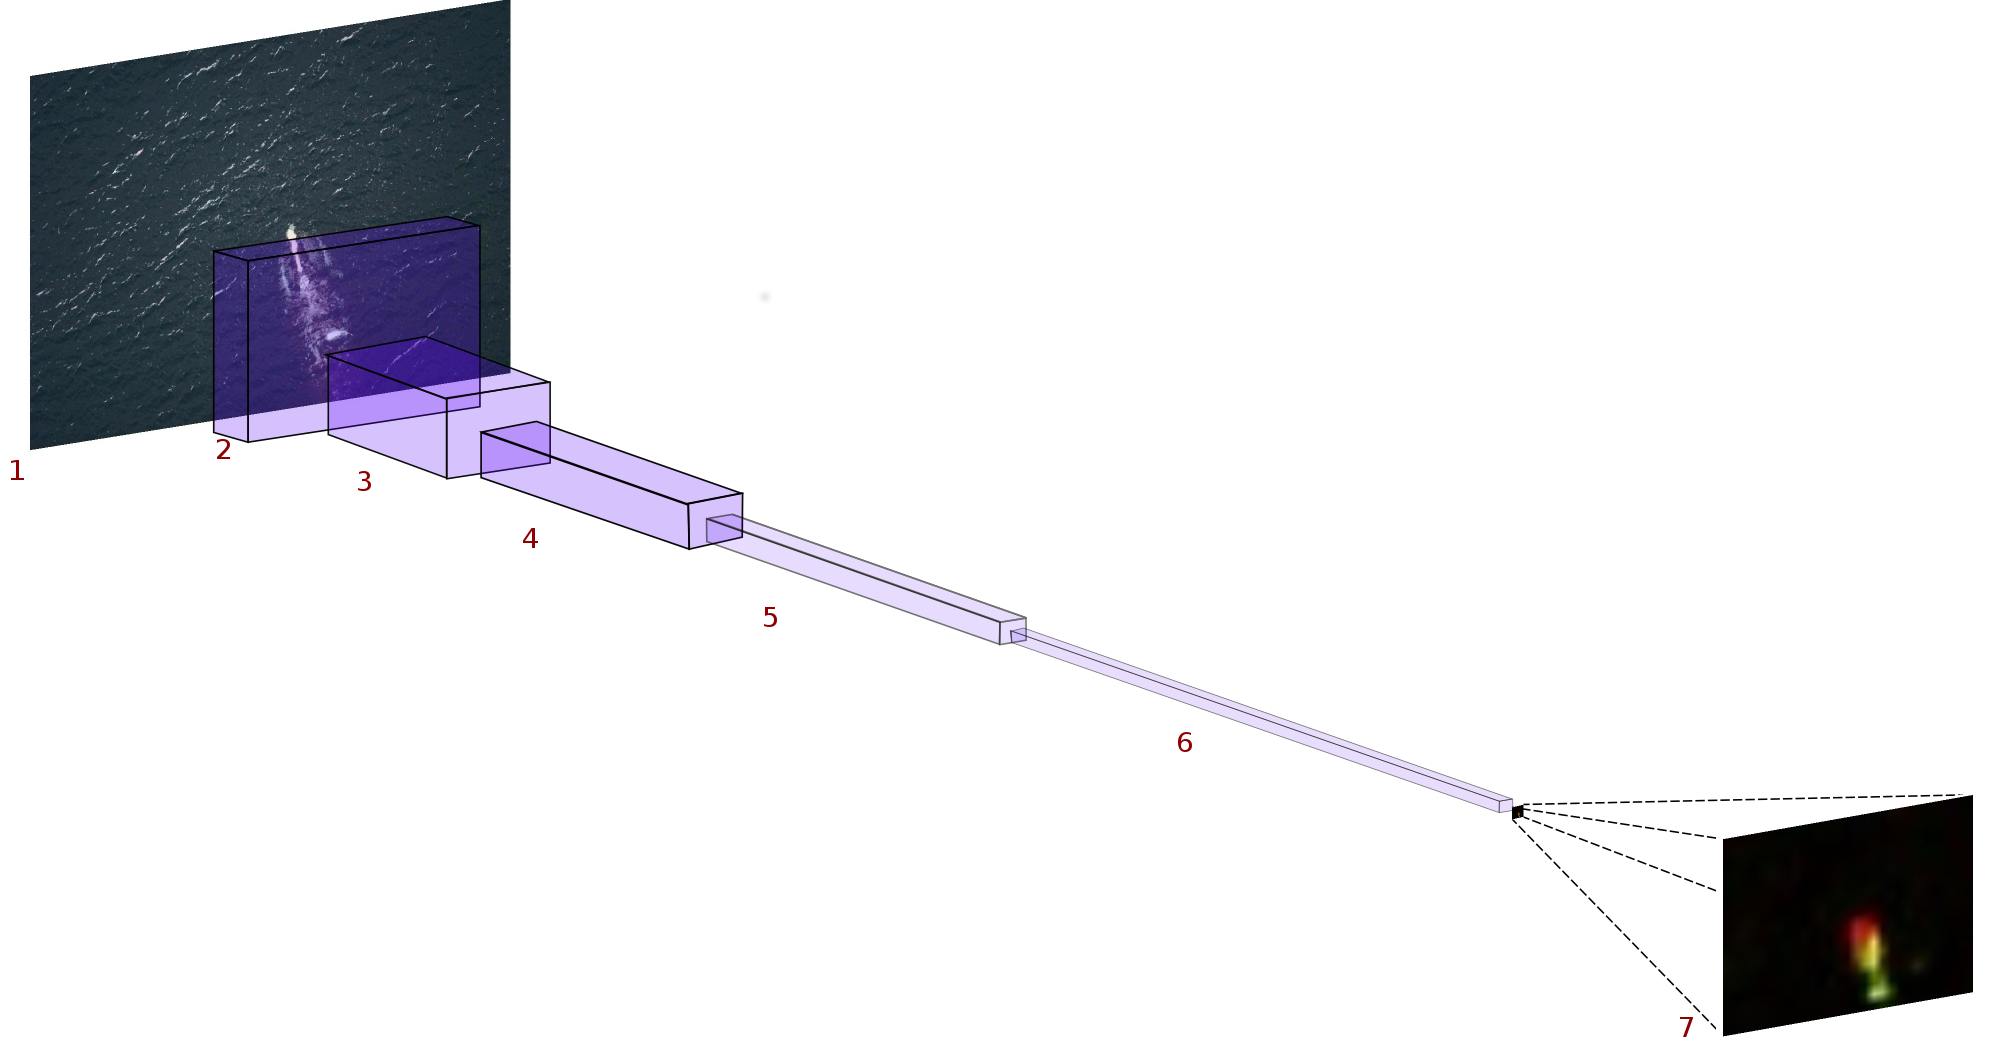
\includegraphics[width=\textwidth]{images/fcn/deconv4.png}
\label{fig:nn}
\caption{Overall architecture of $f_1$.}
\end{minipage}\hfill
\begin{minipage}[t]{.3\textwidth}
\centering
\vspace{20pt}
\begin{tabular}{|c||c|}
\hline
  No. & Shape ($w\times h\times c$) \\
    \hline
    \hline
    $1$ & $900 \times 600 \times 3$   \\
    $2$ & $450 \times 300 \times 48$  \\
    $3$ & $225 \times 150 \times 80$  \\ 
    $4$ & $113 \times 75 \times 112$ \\
    $5$ & $57 \times 38 \times 144$ \\
    $6$ &  $29 \times 19 \times 176$ \\
    $7$ &  $29 \times 19 \times 3$ \\
    \hline
    
\end{tabular}
\captionof{table}{Shape of tensors depicted in figure \ref{fig:nn}}\label{tab:f1shapes}
\end{minipage}
\end{figure}
We train $f_1$ for 20 epochs, using the mean squared error (MSE) as our loss function and the Adam optimization algorithm with an initial learning rate of $0.001$ and batch size of $5$. Together with the MSE we also look at a variant of the S{\o}rensen-Dice coefficient to compare model performance \cite{sorensen1948method}, given by
\begin{align}\label{dice}
\text{QS}(M_i,\hat{M_i})={\frac {2|M_i \cap \hat{M_i}| + 1}{|M_i|+|\hat{M_i}|+1}}.
\end{align}
To artificially increase the size of the dataset we perform random augmentation procedures to each image on the fly; including, flips, rotations, shifts and sheers. However It is well known that a large quantity of varied data is required to train deep networks well, especially to fit complicated functions and generalise well to unseen examples. It is not plausible to learn a huge number of parameters in deep networks reliably in this scenario \cite{zhu2011semi}. Our particular case we hand labelled 700 images, moreover, as can be seen in the particular case of figure \ref{fig:whaleLabel}, they are far from perfect. Large variations in brightness and sea color in $X_i$ ensures even more data is needed to generalize well. 

We combated variation in sea color and brightness by using a histogram matching \cite{gonzalez2002digital} based technique to normalize for such variation. Before each $X_i$ is fed into $f_1$ we match the cumulative distribution function (CDF) of each channel in its YUV color space to a prespecified baseline target image, denoted $T$. 

\begin{figure}[H]
\subfigure[]{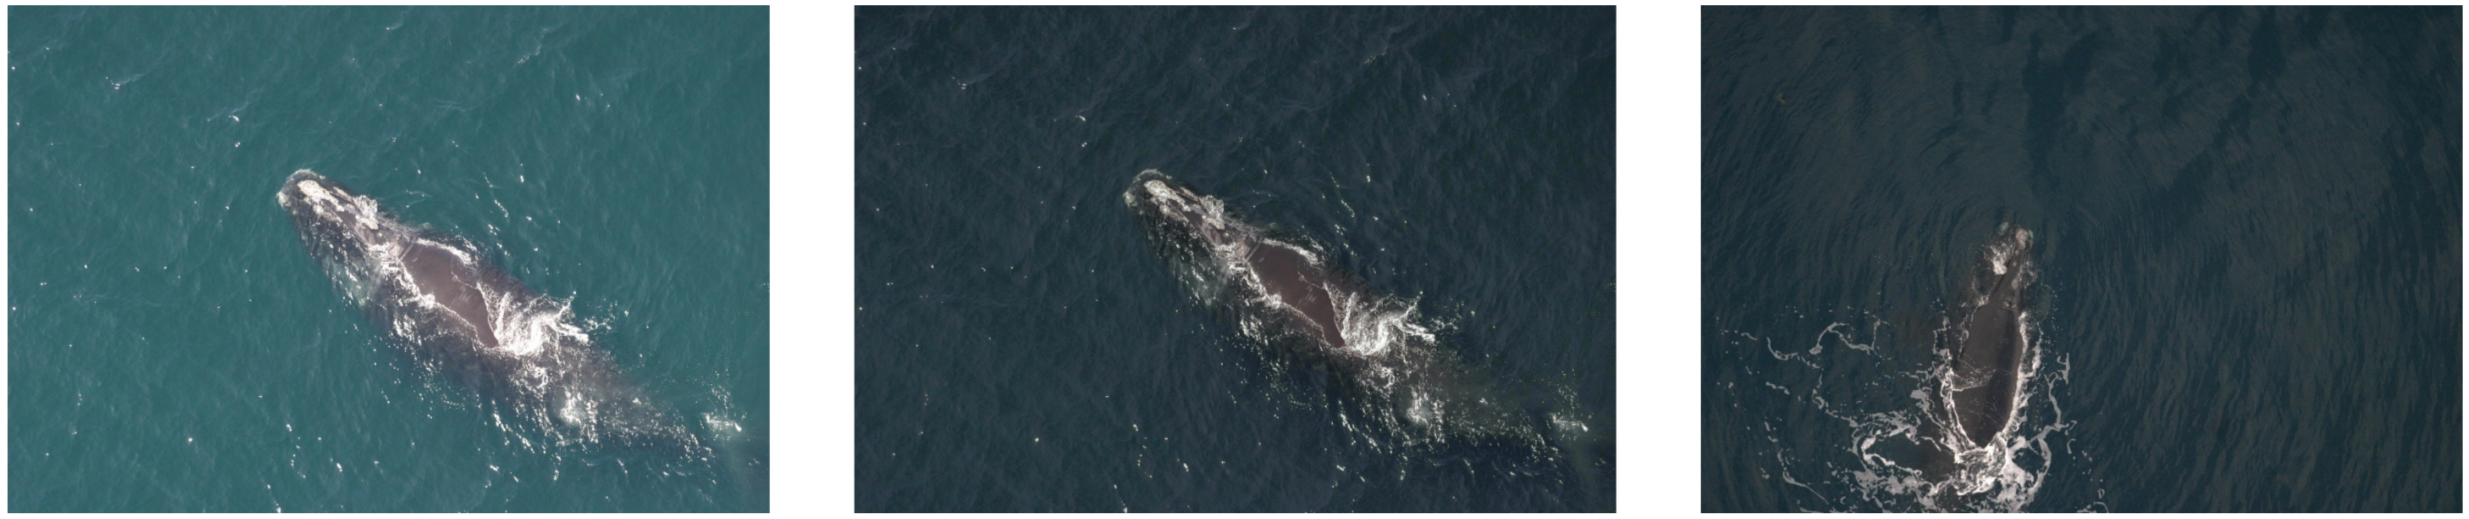
\includegraphics[width=\twoPic\textwidth]{images/histMatch/images.png}}
\subfigure[]{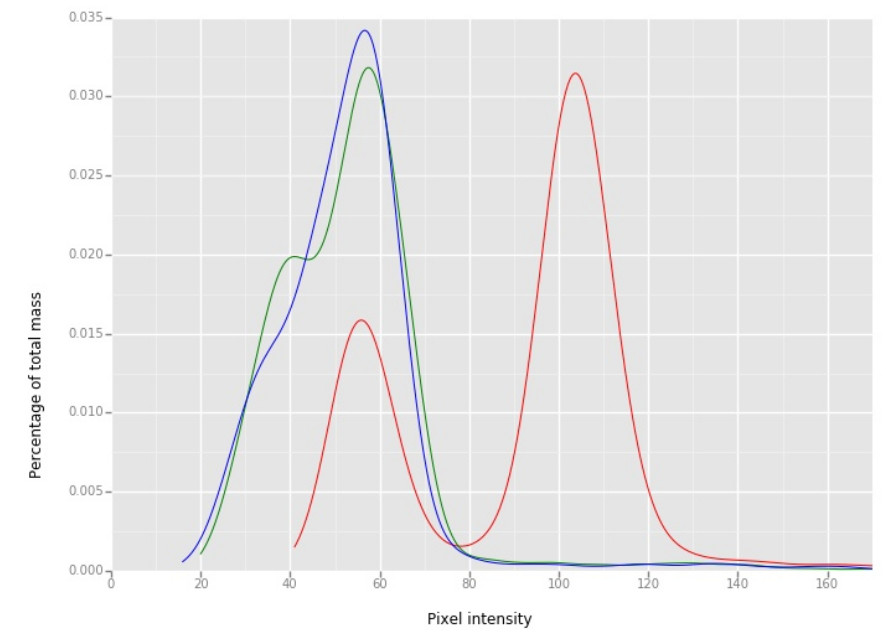
\includegraphics[width=\twoPic\textwidth]{images/histMatch/density.jpg}}
\label{fig:histMatch}
\end{figure}

The results of which are given below in figure \ref{fig:histMatchResults}. As we can see, histogram matching has a positive effect on performance.

\begin{figure}[H]
\begin{center}
\subfigure[]{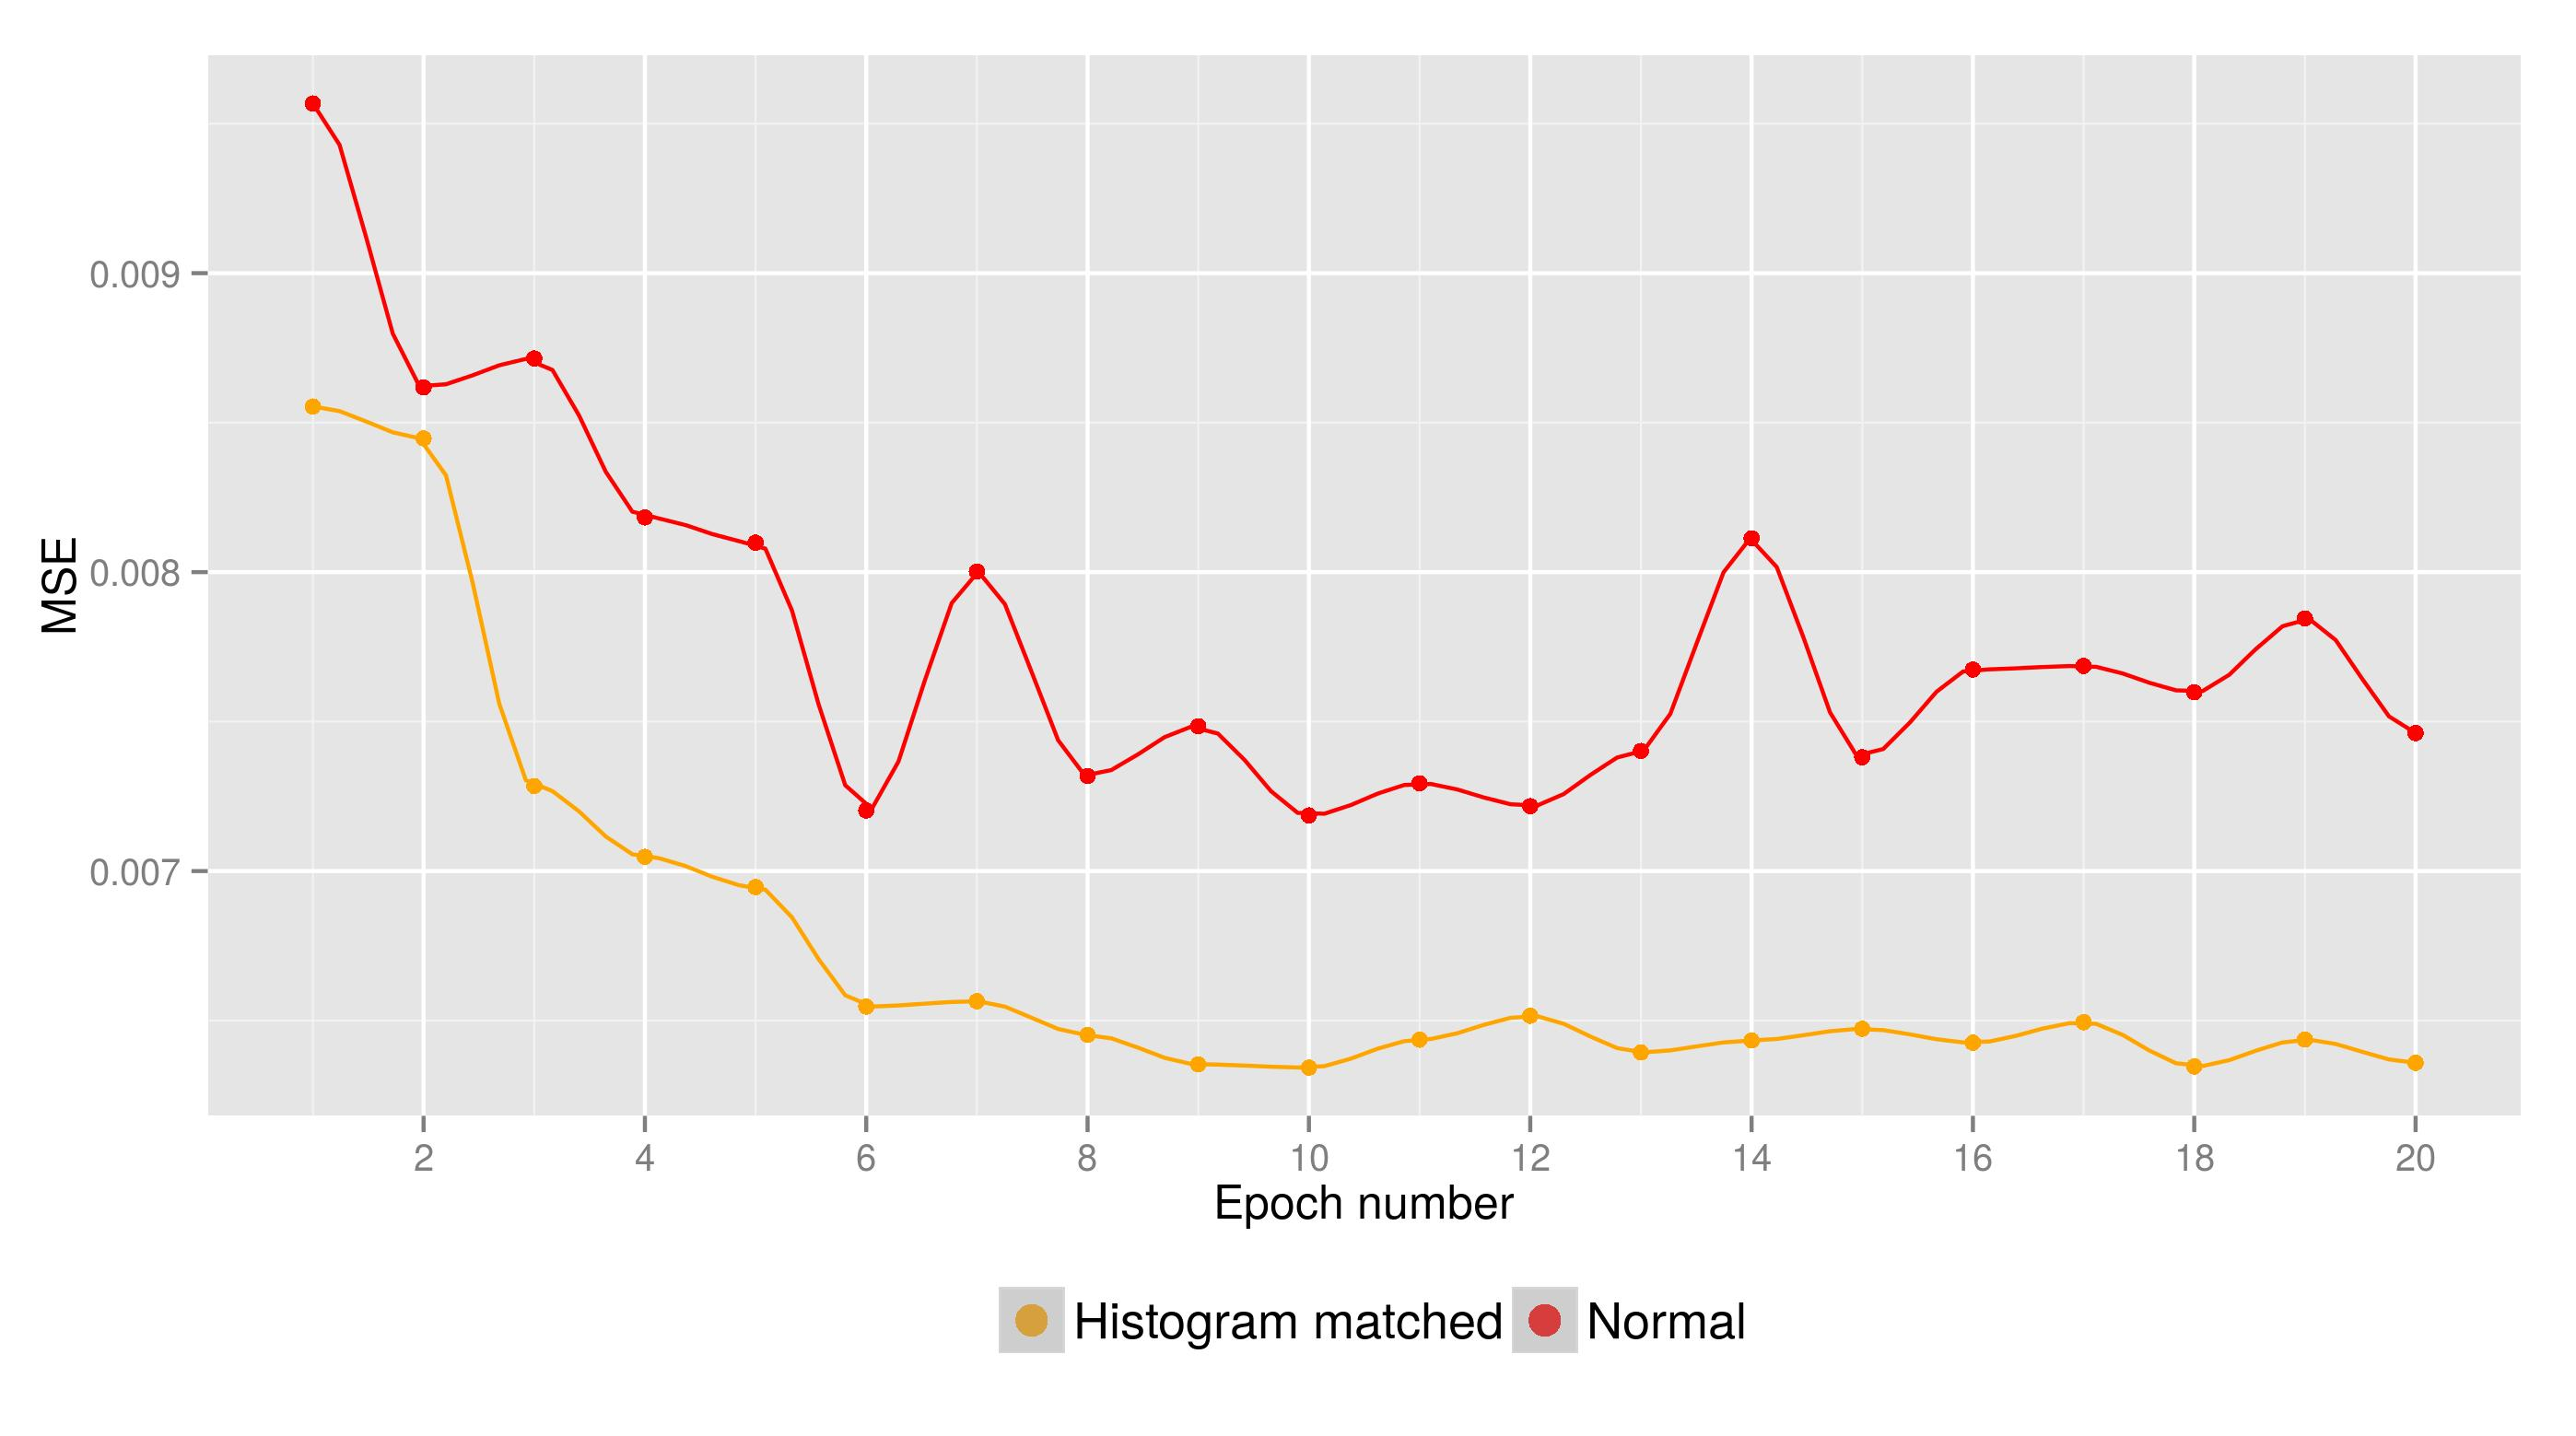
\includegraphics[height=0.25\textwidth ,width=\threePic\textwidth]{results/mse.jpg}}
\subfigure[]{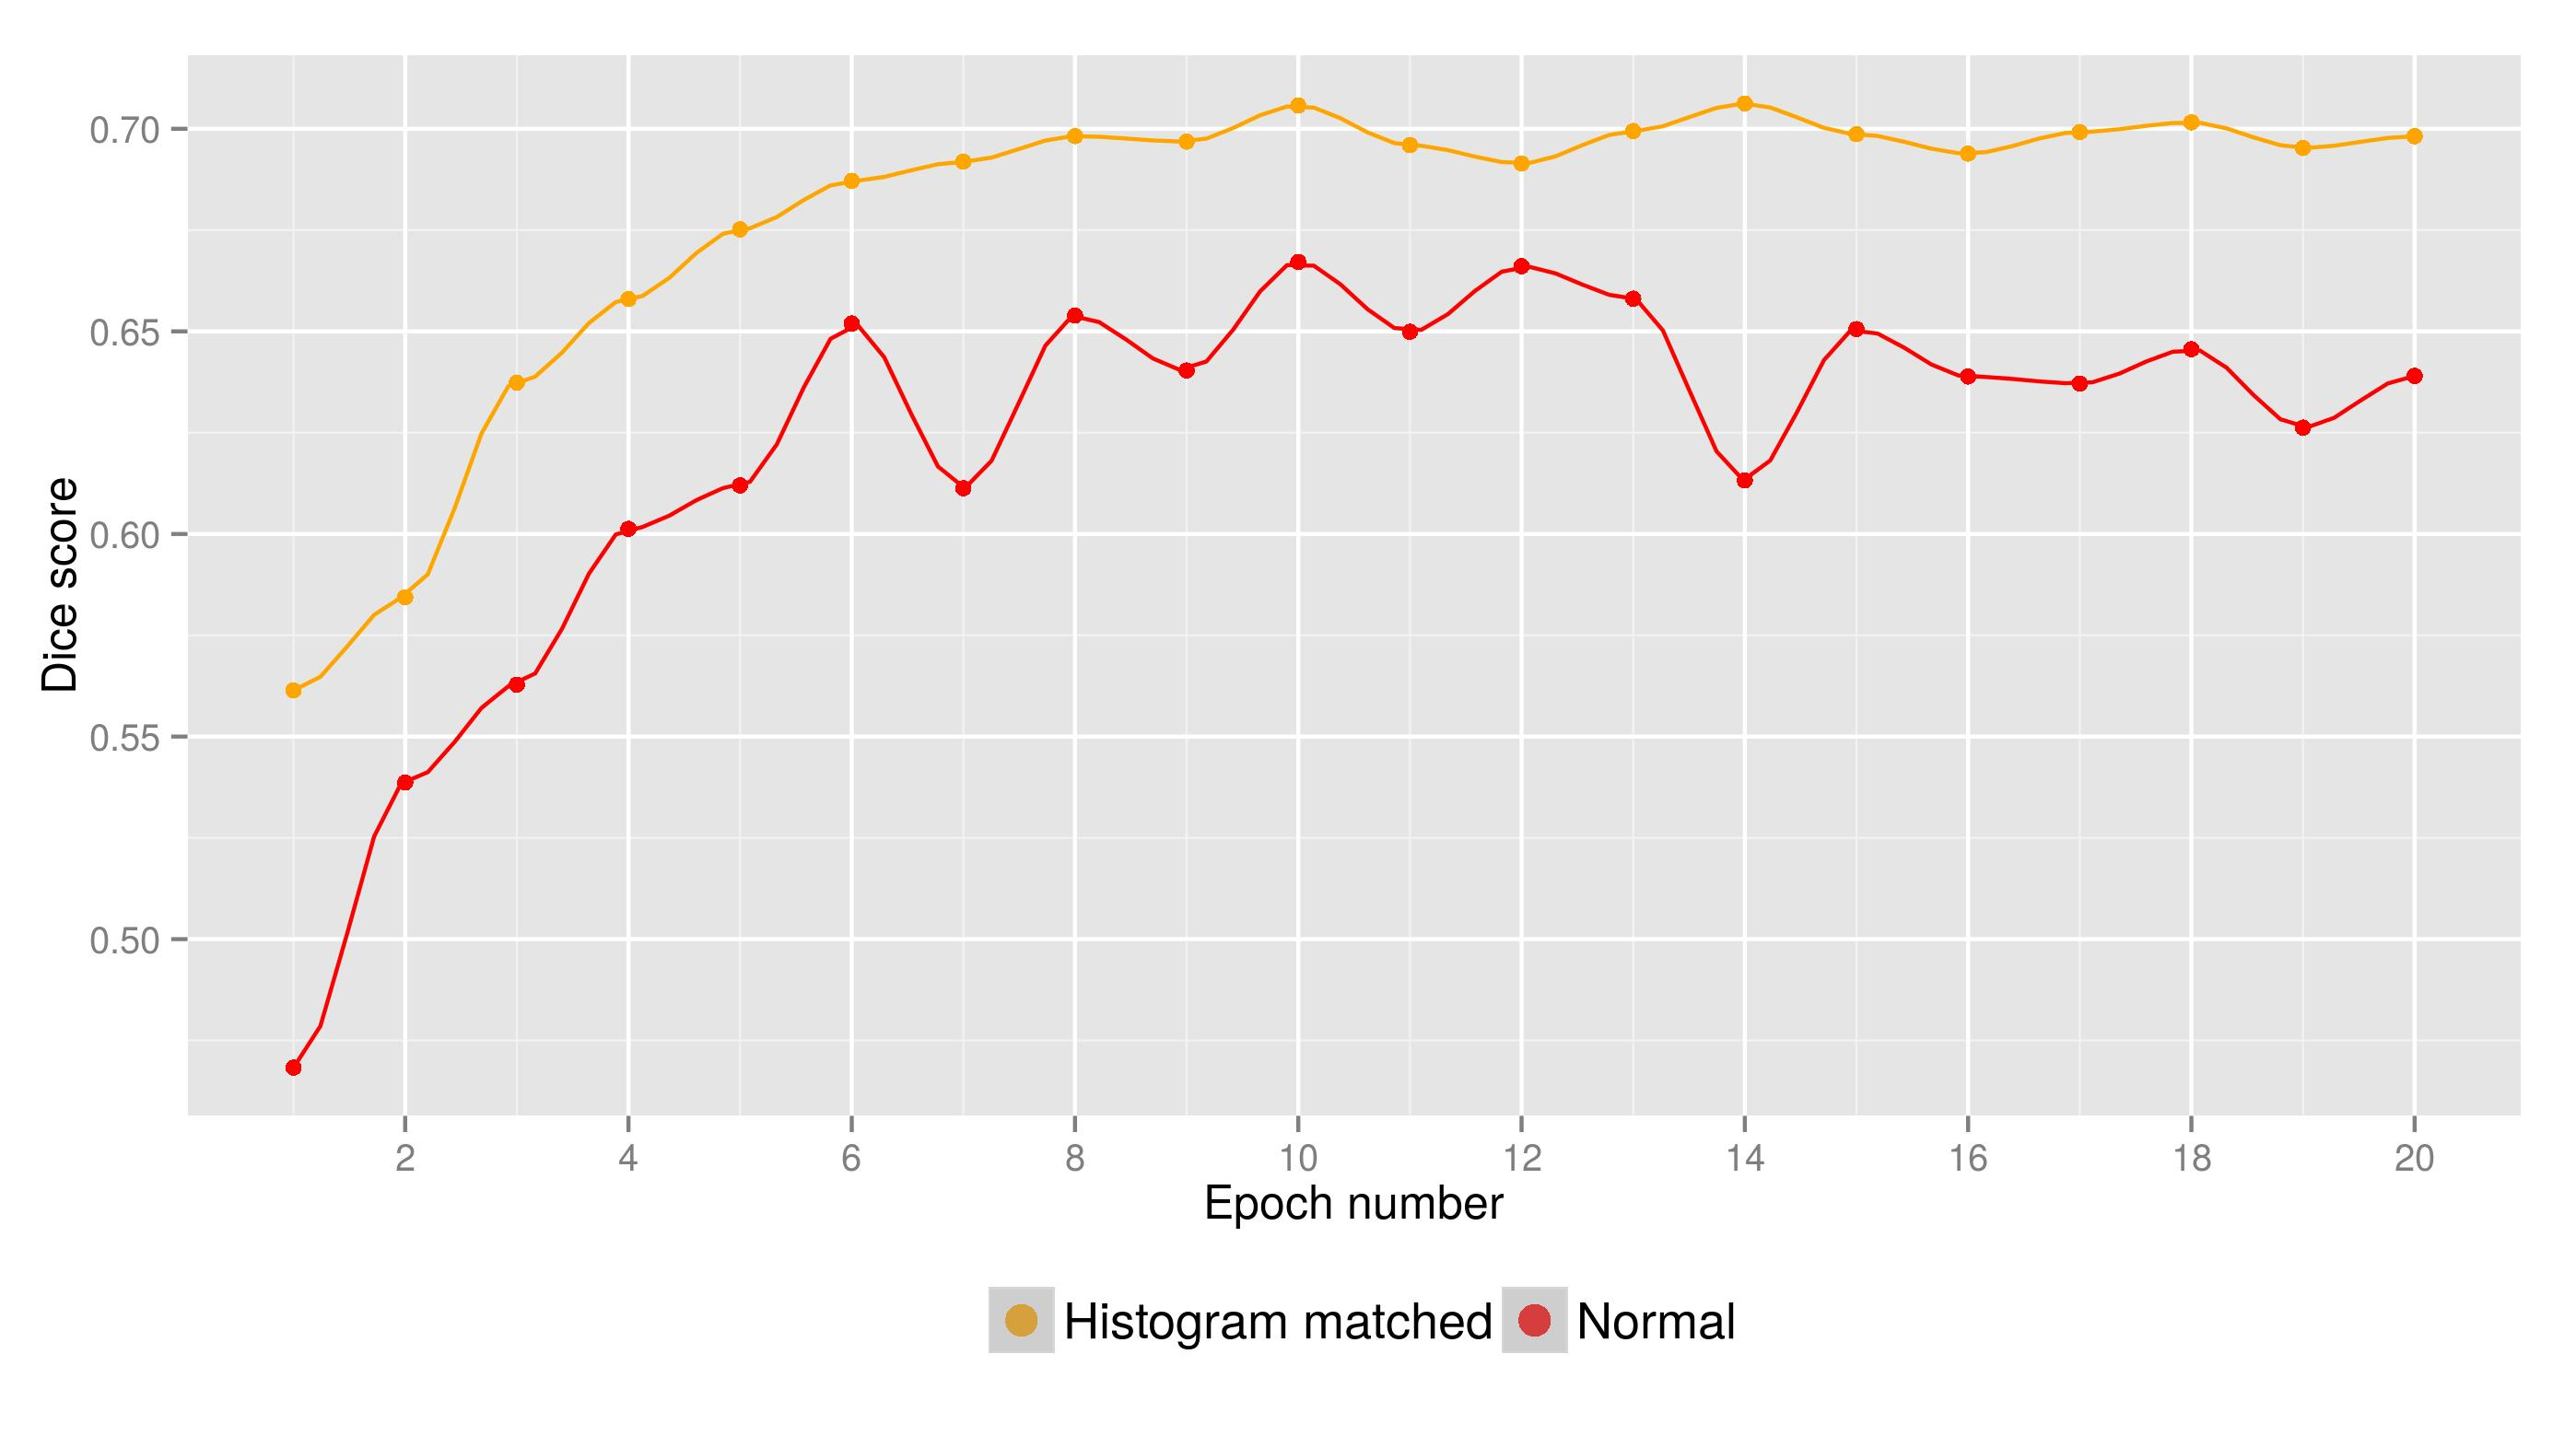
\includegraphics[height=0.25\textwidth ,width=\threePic\textwidth]{results/dice.jpg}}
\subfigure[]{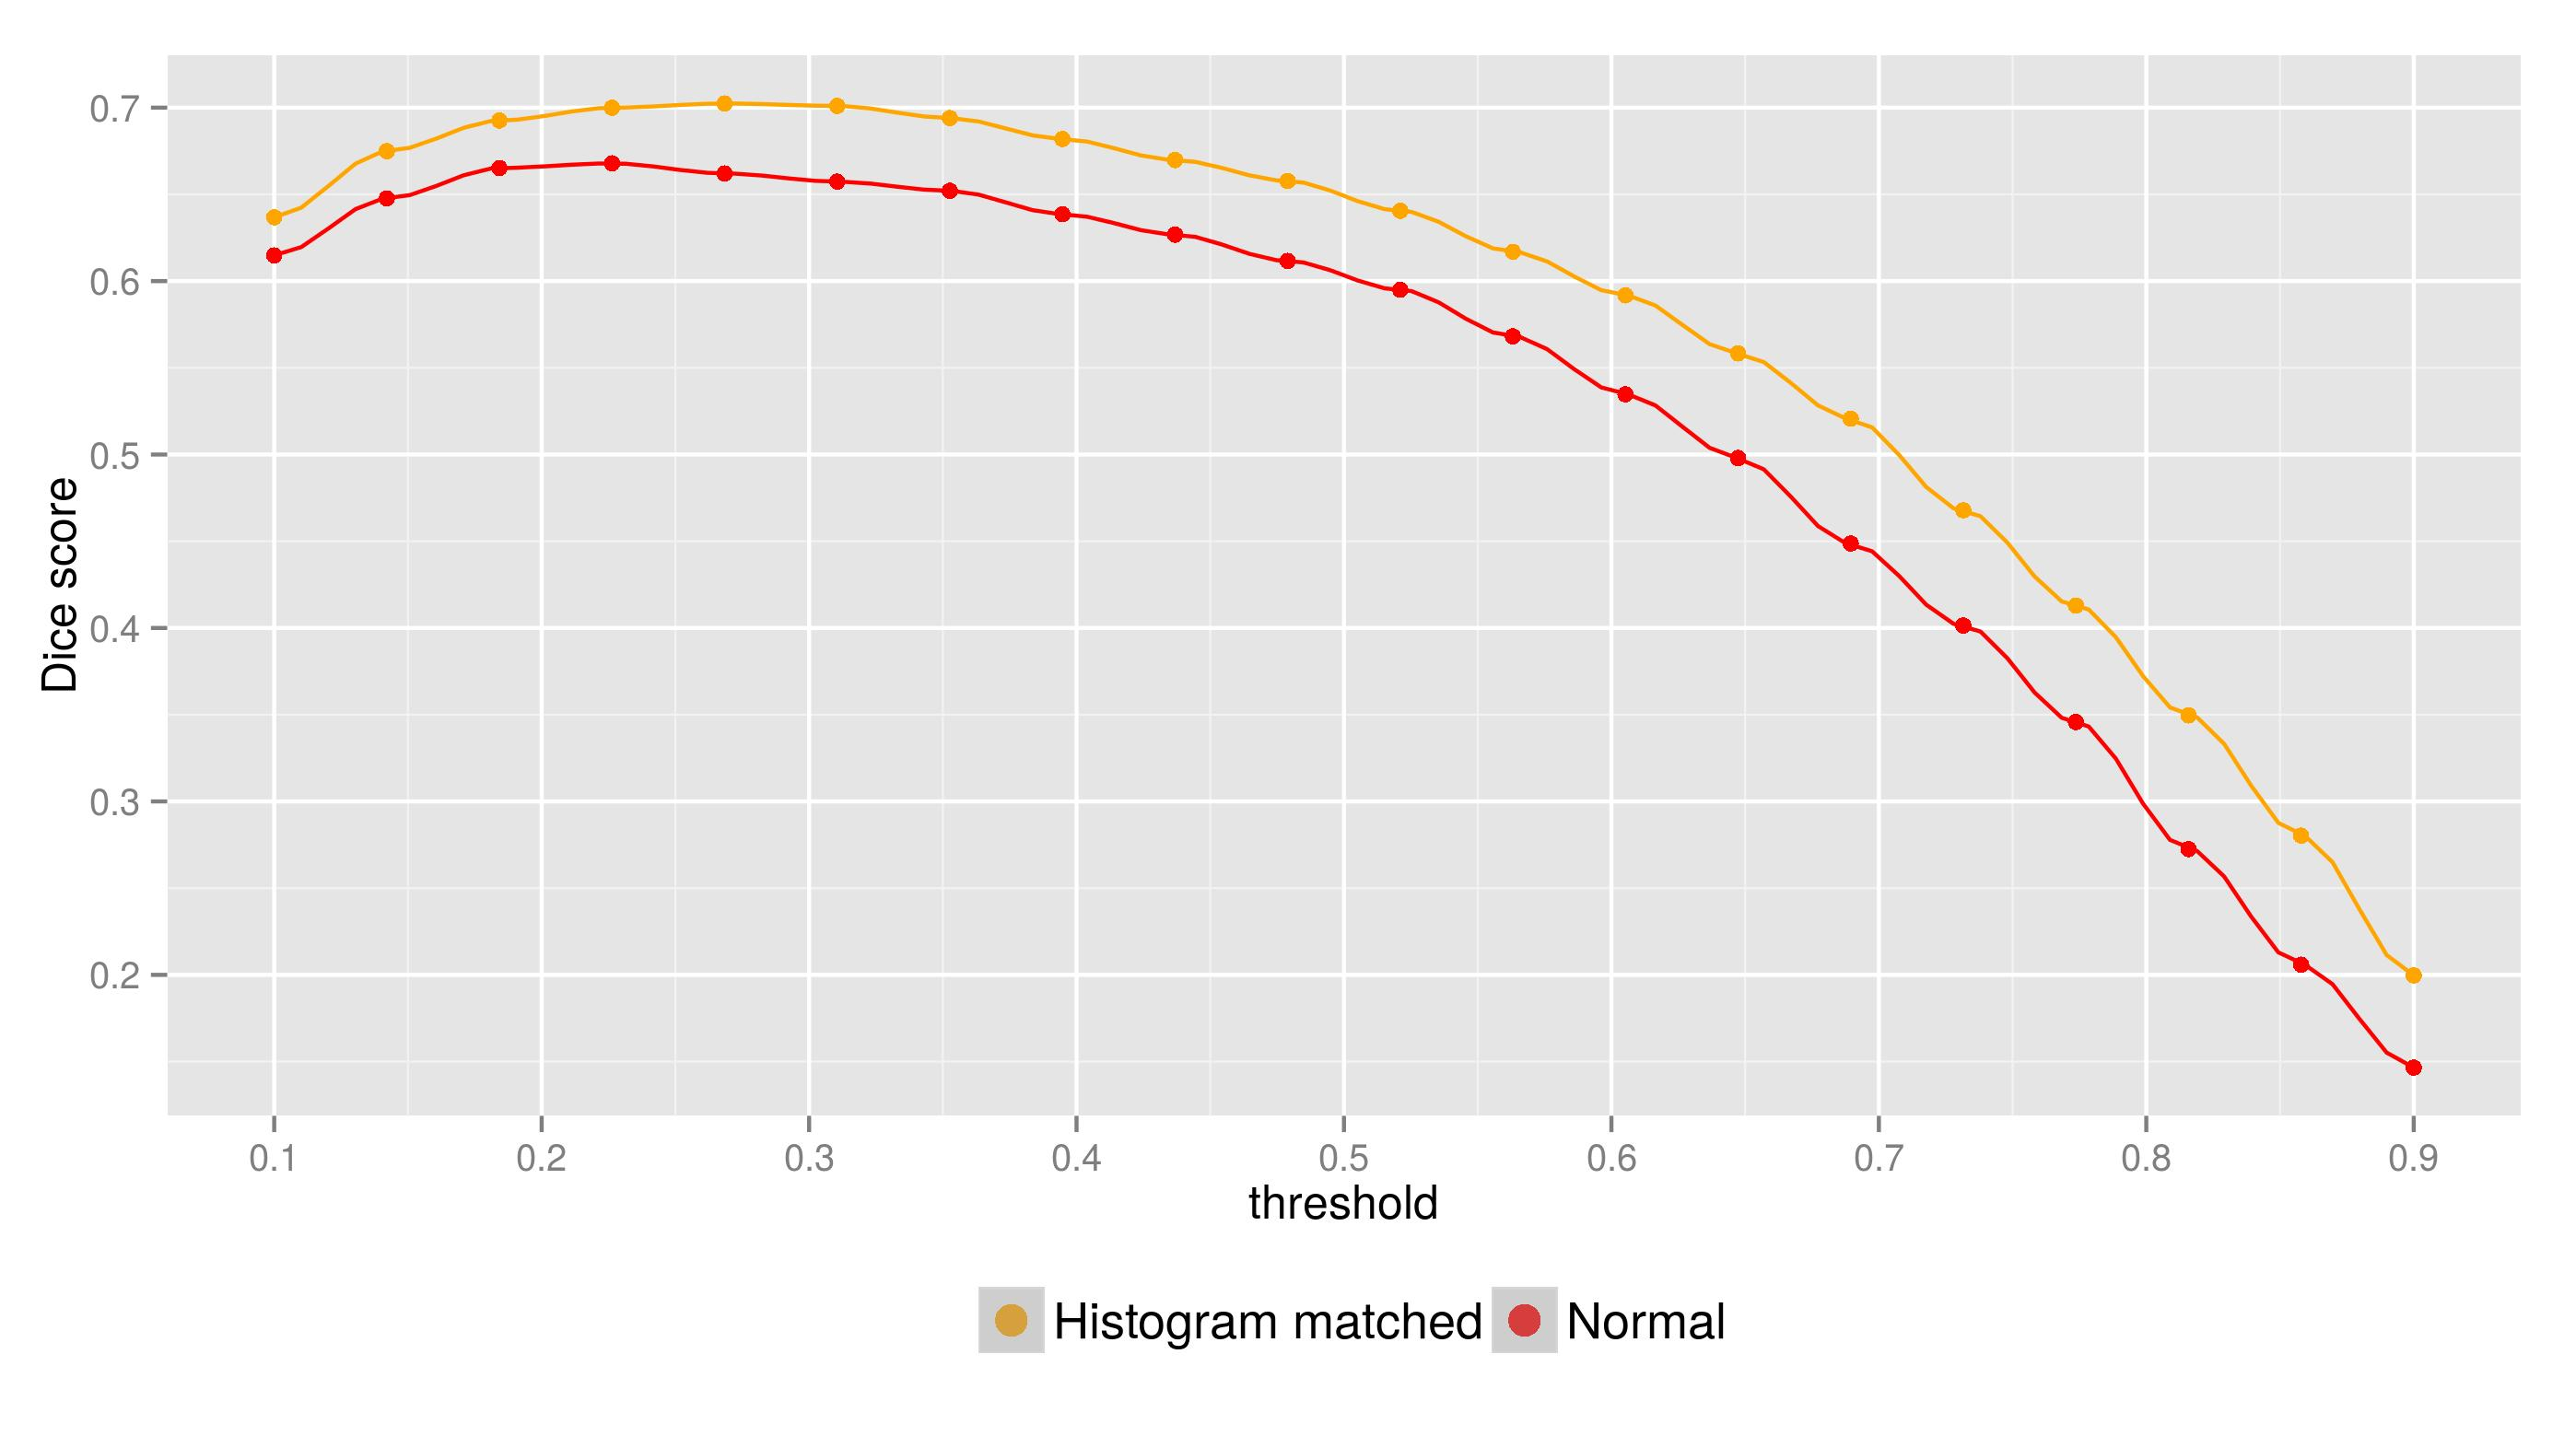
\includegraphics[height=0.25\textwidth ,width=\threePic\textwidth]{results/ROC/dice.jpg}}
\caption{Test performance of $f_1$ for histogram matching and non matching (normal) preprocessing;\
a) MSE per epoch b) Dice score per epoch and c) Dice score over all thresholds after final epoch.
}\label{fig:histMatchResults}
\end{center}
\end{figure}

\subsubsection{Mask post-processing}

We find the largest ellipse of the mask in case more than one whale is in the photo, giving us $\hat{M}_i^{1}$. We then upscale $\hat{M}_i^{1}$ to the same dimensions as $X_i$. To infer direction we find the centroids of the red and green channels, denoted $m_r$ and $m_g$ respectivley. This gives us a vector indicating the direction in which the whale is pointing. To provide robustness to direction we calculate the direction of the first principal axis \cite{hu1962visual}, denoted $u_1 \in \real^2$ . As $u_1$ is an eigenvector we flip its direction if the angle between $u_1$ and $p = m_r - m_g$ is larger than $90\degree$. An example of this is given in figure \ref{fig:maskProcess}.
\begin{figure}[H]
\begin{center}
\foreach \x in {1,2,3,4} 
{
\subfigure[]{\includegraphics[width=\fourPic\textwidth]{images/locator/1/\x .jpg}}
}
\caption{Example of mask post processing stage;\
a) $X_i$, b) $X_i^1$, c) $\hat{M}_i$ and d) $\hat{M}_i^1$ with principal axes illustrated.
}\label{fig:maskProcess}
\end{center}
\end{figure}
We rotate $\hat{M}_i^{1}$ and $X_i$ about $m_r$ by $\theta = \text{atan}2(u_{12},u_{11})$, generating $\hat{M}_i^{2}$ and $X_i^2$. As rotation is completed we want to crop around the head of the whale. The rotated mask $\hat{M}_i^{2}$ is then converted to the HSV color space in order to threshold the hue channel for red and value channel above another tuned threshold as shown in figure \ref{fig:maskRot}.
\begin{figure}[H]
\begin{center}
\foreach \x in {1,4,5,6} 
{
\subfigure[]{\includegraphics[width=\fourPic\textwidth]{images/locator/2/\x .jpg}}
}
\caption{Rotation example in alginment stage;\
a) $X_i$, b) $\hat{M}_i^{1}$, c) $\hat{M}_i^{2}$ and d) $\hat{M}_i^{2}$ thresholded for red.
}\label{fig:maskRot}
\end{center}
\end{figure}
This gives us our head shot $X_i^h$ as shown in figure \ref{fig:origRot}.
\begin{figure}[H]
\begin{center}
\foreach \x in {1,7,8} 
{
\subfigure[]{\includegraphics[width=0.2\textwidth]{images/locator/2/\x .jpg}}
}
\caption{Obtaining the head shot;
a) $X_i$, b) $X_i^{2}$ and c) $X_i^{h}$.
}
\label{fig:origRot}
\end{center}
\end{figure}

\section{Classification}

\subsubsection{Results}

\section{Conclusion}

\section{Figures \& Tables}

The output for figure is:

\begin{figure}[!h]
%\centering\includegraphics{figurename.eps}
%%%call your figure name in the place "figurename.eps"
\caption{Insert figure caption here
\subcaption{a}{Insert Sub caption here}
\subcaption{b}{Insert Sub caption here}}
\label{fig_sim}
\end{figure}


\vskip2pc

\noindent The output for table is:

\begin{table}[!h]
\processtable{An Example of a Table\label{table_example}}%%%Table caption goes here
{\tabcolsep24pt%%%%%%%%% \tabcolsep command is to adjust the inter column spacing of table
\begin{tabular}{|c||c|}%%%The number of columns has to be defined here
\hline
One & Two\\ %%%% Table body
\hline
Three & Four\\%%%% Table body
\hline
\end{tabular}}{}
\end{table}%%%End of the table

\section{Conclusion}
The conclusion text goes here.

\section{Acknowledgment}

Thanks to Christin Khan and Leah Crowe from NOAA for hand labeling the images. 
Kaggle for competition.

\bibliographystyle{IEEEtran}
\bibliography{mybib}
%\vbox{\subsection{Websites}}
%
%\bibitem{bib1}
%
%`Author Guide - IET Research Journals', http://digital-library.theiet.org/journals/author-guide, accessed 27
%November 2014
%
%\bibitem{bib2}
%`Research journal length policy', http://digital-library.theiet.org/files/research\_journals\_\break length\_policy.pdf, accessed 27
%November 2014
%
%\bibitem{bib3}
%`ORCID: Connecting research and researchers', http://orcid.org/, accessed 3 December 2014
%
%\bibitem{bib4}
%`Fundref', http://www.crossref.org/fundref/, accessed 4 December 2014
%
%\vbox{\subsection{Journal articles}}
%
%\bibitem{bib5}
%Smith, T., Jones, M.: 'The title of the paper', IET Syst. Biol., 2007, \textbf{1}, (2), pp. 1--7
%
%\bibitem{bib6}
%Borwn, L., Thomas, H., James, C.,~\textit{et al}.:'The title of the paper, IET
%Communications, 2012, \textbf{6}, (5), pp 125--138
%
%\vbox{\subsection{Conference Paper}}
%
%\bibitem{bib7}
%Jones, L., Brown, D.: 'The title of the conference paper'. Proc. Int.
%Conf. Systems Biology, Stockholm, Sweden, May 2006, pp. 1--7
%
%\vbox{\subsection{Book, book chapter and manual}}
%
%\bibitem{bib8}
%Hodges, A., Smith, N.: 'The title of the book chapter', in Brown, S.
%(Ed.): 'Handbook of Systems Biology' (IEE Press, 2004, 1st edn.), pp. 1--7
%
%\bibitem{bib9}
%Harrison, E.A., and Abbott, C.: 'The title of the book' (XYZ Press,
%2005, 2nd edn. 2006)
%
%\vbox{\subsection{Report}}
%
%\bibitem{bib10}
%IET., 'Report Title' (Publisher, 2013), pp. 1-5
%
%\vbox{\subsection{Patent}}
%
%\bibitem{bib11}
%Brown, F.: 'The title of the patent (if available)'. British Patent
%123456, July 2004
%
%\bibitem{bib12}
%Smith, D., Hodges, J.: British Patent Application 98765, 1925
%
%\vbox{\subsection{Thesis}}
%
%\bibitem{bib13}
%Abbott, N.L.: 'The title of the thesis'. PhD thesis, XYZ University, 2005
%
%\vbox{\subsection{Standard}}
%
%\bibitem{bib14}
%BS1234: 'The title of the standard', 2006
%
%
\section{Appendices}
%
Appendices are allowed but please be aware that these are included in the overall word count.

\end{document}
